\section{Motivation and Background}
\label{sec:background}

\subsection{Motivation}
\label{sec:motivation}

A code assistant deployed for an extended period is rarely trained once and left unchanged. New programming languages and frameworks appear, task requirements shift, and the range of requests a model must handle keeps expanding. Two constraints make this update problem hard in practice. First, full retraining on the union of all data seen so far is computationally expensive and grows more so as the task stream lengthens. Second, data from earlier tasks --- proprietary code, private repositories, or controlled benchmark collections --- may become unavailable or unusable for retraining because of storage or privacy constraints. A practical solution must therefore let the model absorb each new task using only that task's data, while retaining acceptable performance on every task learned previously, and it must do so without knowing in advance which task an incoming request belongs to.

This paper treats sequential code generation as a case study for this problem because the tasks that a code assistant is asked to perform are structurally heterogeneous: some map natural language to code, some map code to code, and some map code to natural language, across many programming languages and syntactic conventions. This heterogeneity means that a continual learning method effective for narrow, homogeneous task streams --- as is common in image classification benchmarks --- does not automatically transfer to code. The remainder of this section introduces the concepts needed to state the problem precisely and to follow the GMM-Router methodology in Section~\ref{sec:methodology}: code language models as the pretrained backbones used throughout this study (Section~\ref{sec:clm_background}), the continual learning problem formulation (Section~\ref{sec:cl_background}), parameter-efficient fine-tuning as the adaptation mechanism (Section~\ref{sec:peft_background}), and Gaussian Mixture Models as the probabilistic tool used for routing (Section~\ref{sec:gmm_background}). Detailed comparison with prior continual learning and routing methods is deferred to Section~\ref{sec:related_work}.

\subsection{Code language models}
\label{sec:clm_background}

Large language models pretrained on source code follow one of two broad architectural families. Encoder-decoder models use a bidirectional encoder together with a causal decoder and are well suited to tasks such as translation and summarization, as in CodeT5 \citep{wang2021codet5} and CodeT5+ \citep{wang2023codet5plus}. Decoder-only models use a single stack of causal self-attention layers that processes both the input and the generated output, which is more natural for open-ended generation and completion; this family includes Code Llama \citep{roziere2023codellama}, StarCoder2 \citep{lozhkov2024starcoder2}, and Qwen2.5-Coder \citep{hui2024qwen25coder}. All of these families are built on the Transformer architecture \citep{vaswani2017attention}. Qwen2.5-Coder, a decoder-only model built for code generation, completion, reasoning, and repair, serves as the backbone throughout this paper (Section~\ref{sec:setup}). Model architecture matters for continual learning because a model updated repeatedly over time must preserve both its representations and its generation abilities across a growing task sequence; this consideration motivates keeping the backbone frozen and confining task-specific updates to a small set of parameters, as described next.

\subsection{Continual learning}
\label{sec:cl_background}

Continual learning --- also called lifelong or sequential learning --- is a setting in which a model is trained on a stream of tasks that arrive one at a time \citep{parisi2019continual,delange2021continual}. Let $\mathcal{T}_1,\ldots,\mathcal{T}_K$ denote a sequence of tasks, each associated with a training dataset
\begin{equation}
    \mathcal{D}_k = \bigl\{(x_i^{(k)},\, y_i^{(k)})\bigr\}_{i=1}^{N_k},
    \label{eq:dataset}
\end{equation}
where $x_i^{(k)}$ is an input prompt and $y_i^{(k)}$ is the target output sequence. The naive sequential update minimizes the current task loss starting from the previous parameters $\theta_{k-1}$: $\theta_k = \arg\min_{\theta}\mathbb{E}_{(x,y)\sim\mathcal{D}_k}[\ell(f_\theta(x),y)]$. This update is simple but typically causes catastrophic forgetting \citep{mccloskey1989catastrophic,kirkpatrick2017overcoming}: updates that reduce loss on the current task overwrite parameters that encoded earlier-task knowledge. In code generation, a model may lose Java-to-C\# translation ability after fine-tuning on Ruby summarization, or degrade on Python generation after adapting to Rust. An effective continual learner must balance stability (retaining earlier tasks) against plasticity (acquiring new ones) \citep{delange2021continual}; this trade-off is pronounced in code, where a task sequence may mix closely related tasks that share useful representations with structurally different tasks that require separate generation behavior. Section~\ref{sec:metrics} defines the Forgetting Measure, Backward Transfer, and Forward Transfer metrics used throughout this paper to quantify this trade-off.

This paper studies the setting in which task identity is not provided at inference time: the model must infer, from the input alone, which adaptation path to use. This requirement motivates the routing formulation developed in Section~\ref{sec:methodology}.

\subsection{Parameter-efficient fine-tuning}
\label{sec:peft_background}

Parameter-efficient fine-tuning (PEFT) methods introduce or modify a small number of trainable parameters while keeping the pretrained backbone frozen, reducing per-task memory and compute cost and making it practical to maintain separate adaptation modules across a growing task sequence. Prompt tuning \citep{lester2021power} prepends a set of trainable continuous embeddings to the input sequence while leaving backbone parameters untouched. Adapter modules \citep{houlsby2019parameter} insert a bottleneck transformation $h' = h + W_{\mathrm{up}}\,\sigma(W_{\mathrm{down}}\,h)$ inside each transformer layer, where $W_{\mathrm{down}}\in\mathbb{R}^{r\times d}$ projects to a bottleneck of size $r\ll d$.

LoRA \citep{hu2022lora}, the PEFT method used throughout this paper, factorizes a weight update into two low-rank matrices:
\begin{equation}
W = W_0 + \Delta W, \qquad \Delta W = \frac{\alpha}{r}BA,
\label{eq:lora}
\end{equation}
where $W_0\in\mathbb{R}^{d\times k}$ is the frozen pretrained weight, $A\in\mathbb{R}^{r\times k}$ and $B\in\mathbb{R}^{d\times r}$ are trainable low-rank factors initialized so that $\Delta W=0$ at the start of training, $r\ll\min(d,k)$, and $\alpha$ is a fixed scaling hyperparameter. LoRA offers a strong balance between efficiency and expressiveness and is easy to insert into attention projection layers. For continual learning, PEFT alone reduces --- but does not eliminate --- interference: a single shared LoRA or prompt can still be overwritten by later tasks. Section~\ref{sec:methodology} uses per-task LoRA experts to remove this source of interference by construction, and combines them with the density-based routing mechanism introduced next.

\subsection{Gaussian Mixture Models}
\label{sec:gmm_background}

A Gaussian Mixture Model (GMM) represents a data distribution as a weighted combination of Gaussian components \citep{bishop2006pattern}. Figure~\ref{fig:gmm_illustration} illustrates a two-component example: the two component densities (dashed) sum to a bimodal mixture density (solid) that a single Gaussian could not represent. For high-dimensional representations it is common to restrict each component's covariance to a diagonal matrix. A diagonal GMM with $M$ components over a representation $\mathbf{z}$ is
\begin{equation}
    p(\mathbf{z}) = \sum_{m=1}^{M} \pi_m\, \mathcal{N}\!\left(\mathbf{z};\, \bm{\mu}_m,\, \operatorname{diag}\!\left(\bm{\sigma}_m^{2}\right)\right),
    \label{eq:gmm}
\end{equation}
where $\pi_m\geq0$, $\sum_{m=1}^{M}\pi_m=1$ are mixture weights, $\bm{\mu}_m\in\mathbb{R}^p$ are component means, and $\bm{\sigma}_m^{2}\in\mathbb{R}^p_{>0}$ collects per-dimension variances. The log-density of a point $\mathbf{z}$ under component $m$ is
\begin{align}
    \log \mathcal{N}\!\left(\mathbf{z};\bm{\mu}_m, \bm{\sigma}_m^2\right)
    ={} & -\frac{1}{2}\Biggl[p\ln(2\pi) + \sum_{j=1}^p \ln \sigma_{mj}^2 \notag \\
    & + \sum_{j=1}^p \frac{(z_j - \mu_{mj})^2}{\sigma_{mj}^2}\Biggr],
    \label{eq:logN}
\end{align}
and the marginal log-density is computed with the log-sum-exp trick for numerical stability:
\begin{equation}
    \log p(\mathbf{z}) = \operatorname{logsumexp}_m\!\left[\log\pi_m + \log \mathcal{N}(\mathbf{z};\bm{\mu}_m,\bm{\sigma}_m^{2})\right].
    \label{eq:logpk}
\end{equation}

\begin{figure}[t]
\centering
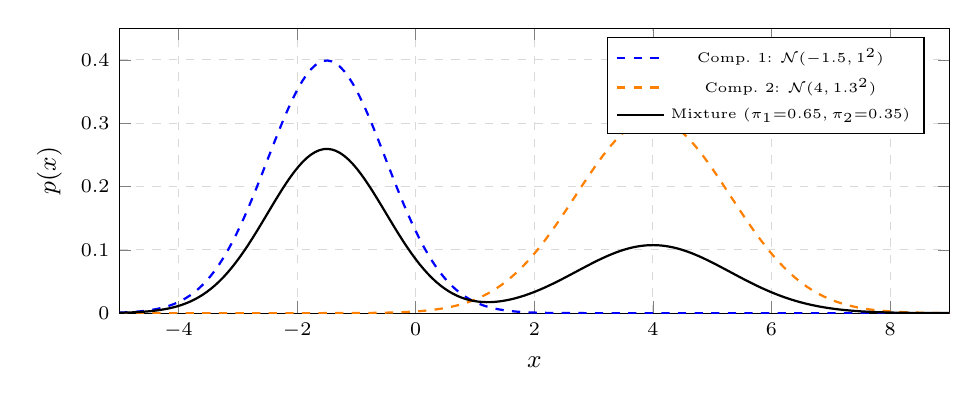
\begin{tikzpicture}
\begin{axis}[
    width=\linewidth, height=5.2cm,
    xlabel={$x$},
    ylabel={$p(x)$},
    xmin=-5, xmax=9,
    ymin=0, ymax=0.45,
    ytick={0, 0.1, 0.2, 0.3, 0.4},
    grid=major,
    grid style={dashed, gray!30},
    legend pos=north east,
    legend style={font=\tiny},
    tick label style={font=\scriptsize},
    label style={font=\small},
]
\addplot[blue, dashed, thick, domain=-5:9, samples=200]
    {1/sqrt(2*pi) * exp(-0.5*(x+1.5)^2)};
\addplot[orange, dashed, thick, domain=-5:9, samples=200]
    {1/sqrt(2*pi*1.69) * exp(-(x-4)^2/(2*1.69))};
\addplot[black, thick, domain=-5:9, samples=200]
    {0.65/sqrt(2*pi) * exp(-0.5*(x+1.5)^2)
     + 0.35/sqrt(2*pi*1.69) * exp(-(x-4)^2/(2*1.69))};
\addlegendentry{Comp.\ 1: $\mathcal{N}(-1.5,1^2)$}
\addlegendentry{Comp.\ 2: $\mathcal{N}(4,1.3^2)$}
\addlegendentry{Mixture ($\pi_1{=}0.65,\pi_2{=}0.35$)}
\end{axis}
\end{tikzpicture}
\caption{A two-component Gaussian Mixture Model. Each dashed curve is an individual component; the solid curve is their weighted sum. The mixture density is bimodal, whereas a single Gaussian would be forced to place mass between the two clusters.}
\label{fig:gmm_illustration}
\end{figure}

Because component assignment is a latent variable, GMM parameters are fitted by maximum likelihood using Expectation-Maximization (EM) \citep{dempster1977maximum}. The E-step computes the responsibility of component $m$ for observation $\mathbf{z}_i$,
\begin{equation}
    r_{im} = \frac{\pi_m \, \mathcal{N}(\mathbf{z}_i;\bm{\mu}_m,\bm{\sigma}_m^2)}{\sum_{m^\prime} \pi_{m^\prime}\,\mathcal{N}(\mathbf{z}_i;\bm{\mu}_{m^\prime},\bm{\sigma}_{m^\prime}^2)},
    \label{eq:resp}
\end{equation}
and the M-step updates parameters using effective counts $N_m=\sum_i r_{im}$:
\begin{align}
    \pi_m &= \frac{N_m}{N}, \qquad
    \bm{\mu}_m = \frac{1}{N_m}\sum_{i=1}^N r_{im}\mathbf{z}_i, \\
    \sigma_{mj}^2 &= \max\!\left(\frac{\sum_{i=1}^N r_{im}(z_{ij}-\mu_{mj})^2}{N_m},\sigma^2_{\min}\right),
    \label{eq:var_update}
\end{align}
where $\sigma^2_{\min}>0$ is a variance floor that prevents component collapse. Algorithm~\ref{alg:em_gmm} summarizes the procedure, alternating the E-step (Eq.~\eqref{eq:resp}) and the M-step (Eq.~\eqref{eq:var_update}) until the average log-likelihood converges.

\begin{algorithm}[t]
\caption{Expectation-Maximization for a Diagonal GMM}
\label{alg:em_gmm}
\KwIn{Observations $\{\mathbf{z}_i\}_{i=1}^N$; components $M$;\\ tolerance $\delta$; max steps $T_{\max}$}
\KwOut{Fitted $\{\pi_m, \bm{\mu}_m, \bm{\sigma}_m^2\}_{m=1}^M$}
Initialize $\pi_m \leftarrow 1/M$; sample $\bm{\mu}_m$ uniformly from $\{\mathbf{z}_i\}$; set $\bm{\sigma}_m^2$ to the global per-dimension variance\;
$\mathcal{L}^{(0)} \leftarrow -\infty$\;
\For{$t = 1, \ldots, T_{\max}$}{
    \textbf{E-step:} compute $r_{im}$ for all $i,m$ via Eq.~\eqref{eq:resp}\;
    \textbf{M-step:} update $\pi_m,\bm{\mu}_m,\bm{\sigma}_m^2$ for all $m$ via Eq.~\eqref{eq:var_update}\;
    $\mathcal{L}^{(t)} \leftarrow (1/N)\sum_{i=1}^N \log p(\mathbf{z}_i)$ via Eq.~\eqref{eq:logpk}\;
    \If{$|\mathcal{L}^{(t)} - \mathcal{L}^{(t-1)}| < \delta$}{\textbf{break}}
}
\Return $\{\pi_m, \bm{\mu}_m, \bm{\sigma}_m^2\}_{m=1}^M$\;
\end{algorithm}

GMM-based routing decides which adaptation module to apply to a given input by estimating how likely its feature representation is under each task's fitted density; this connects to the mixture-of-experts literature, in which a gating function assigns inputs to specialized expert networks \citep{jacobs1991adaptive,jordan1994hierarchical,shazeer2017outrageously,fedus2022switch}, reviewed further in Section~\ref{sec:related_work}. In the code domain, a single task often contains diverse subtypes --- algorithmic problems, string processing, data-structure manipulation --- that a single Gaussian cannot represent well; a mixture captures several sub-regions within the same task, and evaluating each task's fitted GMM on a frozen, task-agnostic representation provides a routing score without requiring task labels at inference time, motivating the routing mechanism developed in Section~\ref{sec:methodology}.
